\chapter{An Introduction to Kirby Calculus}
This chapter introduces basic notions of Kirby calculus and related topics. For a complete and detailed introduction, we refer the reader to the Gompf and Stipsicz's book \cite{gompf1999four} and Akbulut's book \cite{akbulut2001four}.
Kirby calculus, named after Robion Kirby, is a diagrammatic tool for studying $4$-manifolds.
\section{Anatomy of a $4$-Manifold}
Let $X$ be an orientable, connected $4$-manifold. We assume the reader is familiar with handle decompositions and Morse functions. For an introduction, consult \cite{benedetti2019lectures}. \\
Consider an ordered handle decomposition of $X$. Since $X$ is connected, handle cancellation ensures we can reduce the handle decomposition to include only one $0$-handle. Applying the same procedure to the dual handle decomposition results in a handle decomposition with only one $0$-handle and one $4$-handle.
Denoting by $n_i$ the number of $i$-handles $i=0,\dots 4$, we write: $$
X = H_0 \cup H_1^1 \cup \dots \cup H_1^{n_1}\cup H_2^1
\cup\dots\cup H_2^{n_2}\cup H_3^1\cup \dots \cup H_3^{n_3} \cup H_4$$
Our strategy involves drawing the attaching region schematically. Start with $1$-handles $H_1 = \D^0 \times \D^4$, which are attached to $$
\partial \D^4 = \s^3 = \R^3 \cup \{\infty\}
$$
The attaching region is $\s^0 \times \D^3 = \{-1, 1\}\times \D^3$.
There is a unique way to attach them to make the resulting manifold orientable.
We remove two balls from $\R^3$, and we identify their boundaries through a reflection. We represent the whole attaching region, as in Figure \ref{fig:kiuby}(a).
Observe that $$
H_0 \cup H_1^1 \cup \dots \cup H_1^{n_1} = \natural_1^{n_1}(\s^1 \times \D^3)
$$After all the $1$-handles are attached, the resulting boundary becomes: $$Y = \#_1^{n_1}(\s^1 \times \s^2)$$
The attaching spheres of the $2$-handles form a link $L$ in $Y$. To describe the $2$-handle attachment, we use framings. Since every $3$ manifold is parallelizable, \cite{benedetti2019lectures}, we can arbitrarily choose a trivialization of $\nu(L)$. After this choice, the trivializations of $\nu(L) \cong L \times \D^2$ are classified by $$
\pi_1(O(2)) \cong \Z
$$Each component of $L$ is assigned an integer, specifying the framing. Figure \ref{fig:kiuby}(b) is an example of a Kirby diagram.
\begin{figure}[H]
    \centering
    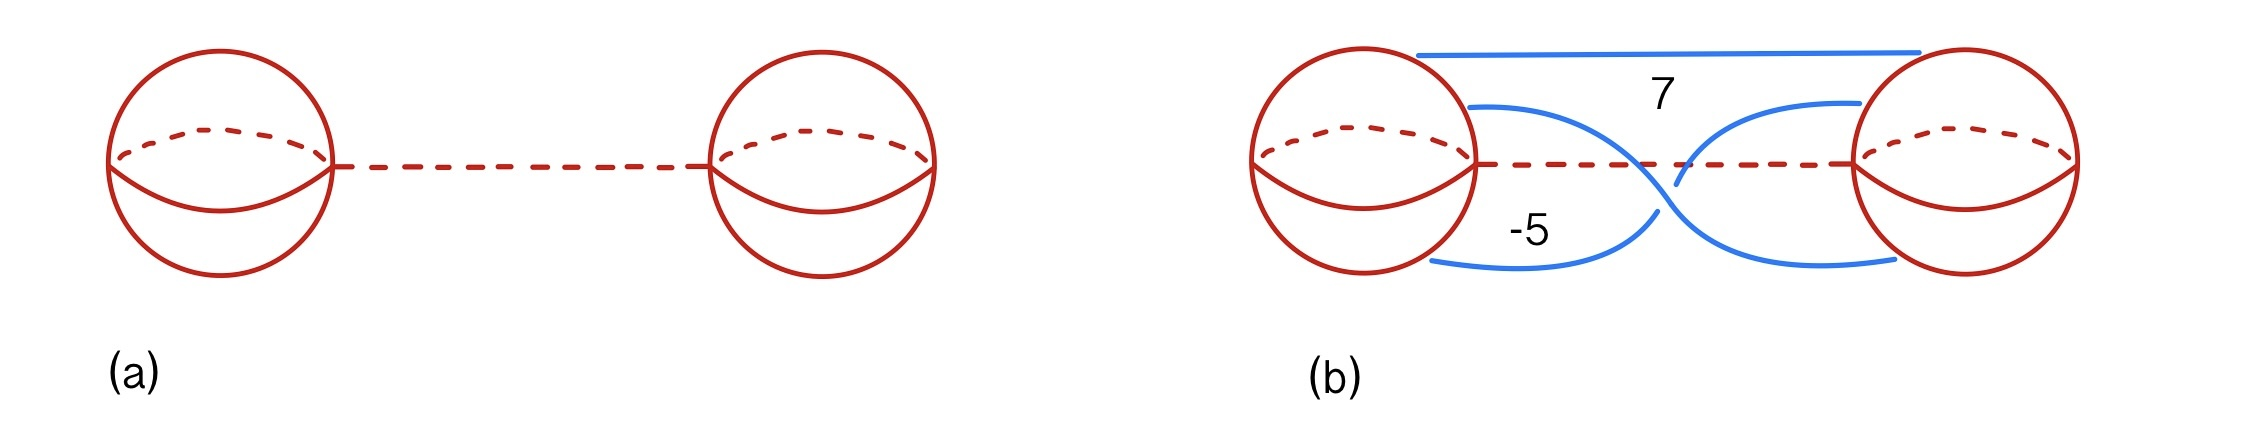
\includegraphics[scale=0.2]{figures/kiuby.jpeg}
    \caption{A $1$-handle on the left, a Kirby diagram on the right}
    \label{fig:kiuby}
\end{figure}
\begin{cla}
If $X$ is closed, the attachment of $3$-handles is immaterial.
\end{cla}
Indeed, examining the dual handle decomposition, we find $$
\partial (\B^4 \cup_1^{n_1} H_1^i \cup_1^{n_2} H_2^j) = \#_1^{n_3}(\s^1 \times \s^2)
$$and $n_3 = n_1$. 
\begin{thm}(Laudenbach, Poenaru) \\
Every self diffeomorphism of $\#_1^k(\s^1 \times \s^2)$ extends to a self diffeomorphism of $\natural_1^k(\s^1 \times \D^3)$
\end{thm}
As a result, there is a unique way to finish building $X$ from $(\B^4 \cup_1^{n_1} H_1^i \cup_1^{n_2} H_2^j)$, by attaching $3$ and $4$-handles.
\section{Drilling out Disks}\label{driii}
In this section, we introduce Akbulut's notation for $1$-handles, called the dotted circle notation. While doing that, we explain how to find the Kirby diagram of a unknotted disk complement in $\B^4$. \\ \\
Consider $X \cup H_1$. If $X$ is connected, we can recover $X$ by gluing a $2$-handle. Then, we can dismantle the $2$-handle by carving a disk, that means drilling out a open tubular neighbourhood of a properly embedded disk.
As a result, attaching a $1$-handle to $\B^4$, is the same as removing a disk
$D$ from $\B^4$, with $\partial D \subseteq \s^3$.
This allows us to represent a $1$-handle as a boundary of the carved disk, marked with a dot\footnote{This is only to distinguish $1$ and $2$-handles}. 

\section{Kirby Moves}
After introducing the combinatorial objects, which are Kirby diagrams, we proceed by introducing a set of moves, called Kirby moves. We translate the well known moves on handle decompositions, into the language of Kirby diagrams. For convenience, we use Akbulut's notation.  \\ 
\textbf{1-handle slide}: 
We slide a $1$-handle over the other, as in Figure \ref{fig:hs1}.
\begin{figure}[H]
    \centering
    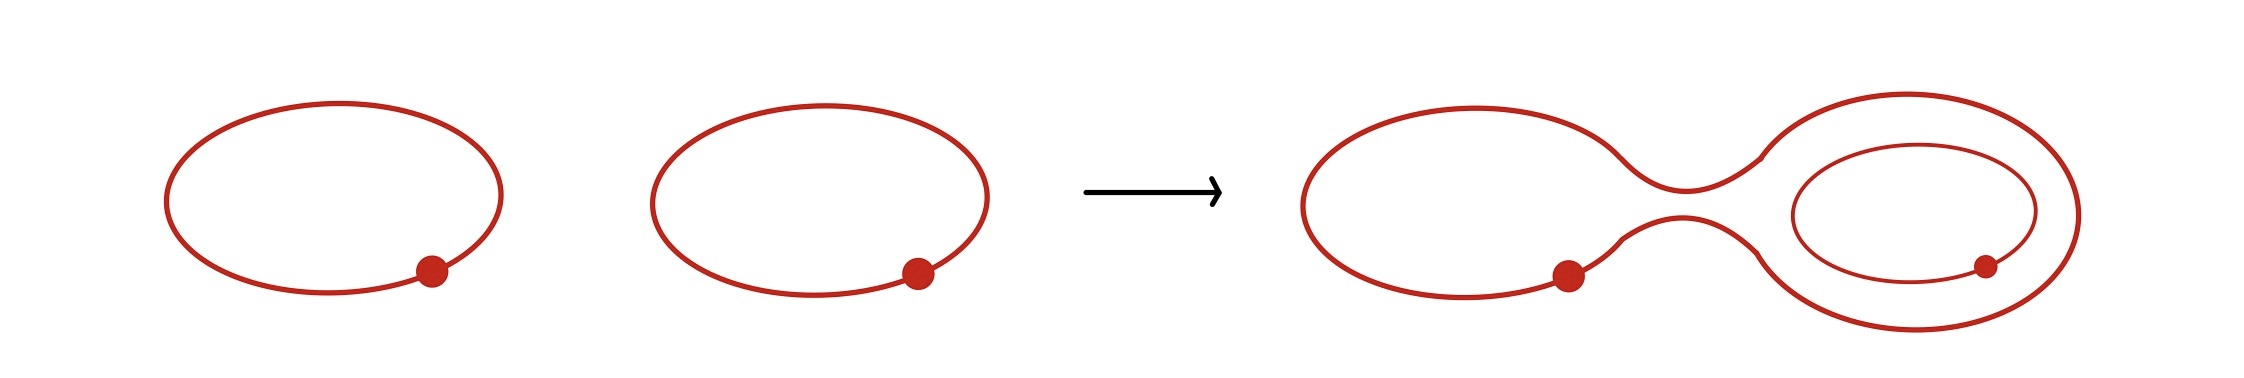
\includegraphics[scale=0.2]{figures/hs1.jpeg}
    \caption{A $1$-handle slide}
    \label{fig:hs1}
\end{figure}
\textbf{2-handle slide}:
Suppose we want to slide $K_1$ over $K_2$. We consider a parallel copy $K_2'$ of $K_2$ and then we perform the connect sum $K_1 \#K_2'$. The new framing on $K_2$ is: $$
f_{K_1}+f_{K_2} + 2lk(K_1, K_2)
$$
\begin{figure}[H]
    \centering
    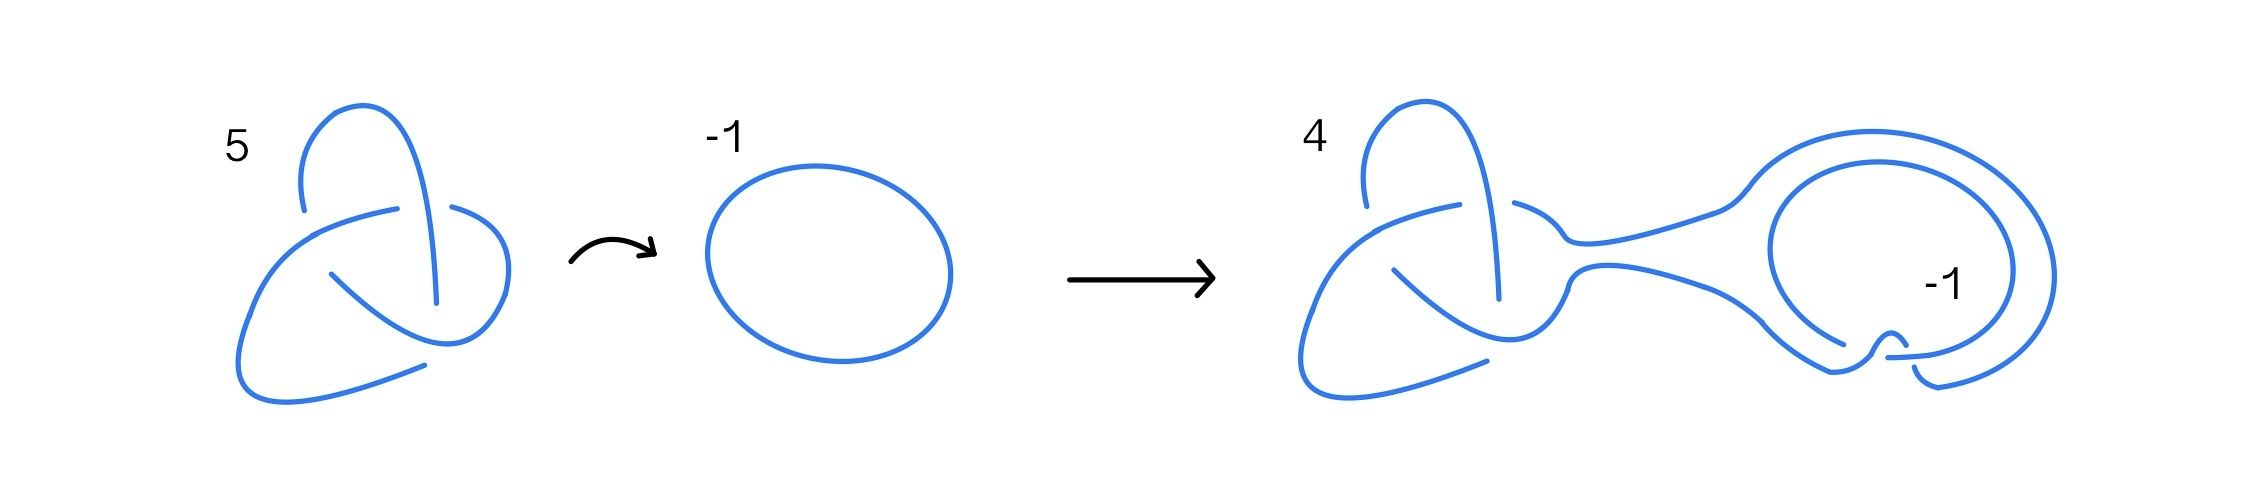
\includegraphics[scale=0.2]{figures/hs2.jpeg}
    \caption{A $2$-handle slide}
    \label{fig:hs2}
\end{figure}
\textbf{Handle creation and cancellation of complementary pairs}: \\
Suppose that the attaching sphere of a $2$-handle transversally intersects the belt sphere of a $1$-handle in one point. Then we can perform a handle cancellation. Its inverse is called handle creation. \\
These moves don't change the manifold represented by a Kirby diagram, up to diffeomorphisms. Moreover the following theorem holds.
\begin{thm} Let $X$ be a closed $4$-manifold. Any two Kirby diagrams of $X$ are related by a finite sequence of isotopies and Kirby moves. 
\end{thm}
\section{The Light Bulb Trick}
In the next chapters, we manipulate knots and core curves inside Kirby diagrams. In particular, it will be useful to unlink a knot $K$ from the attaching curve of a $2$-handle. \\ \\
If such a core curve is a $0$-framed unlink, then we just perform a number of handle slides for each time $K$ passes through the blue circle, as depicted in Figure \ref{fig:squish}.
\begin{figure}[H]
    \centering
    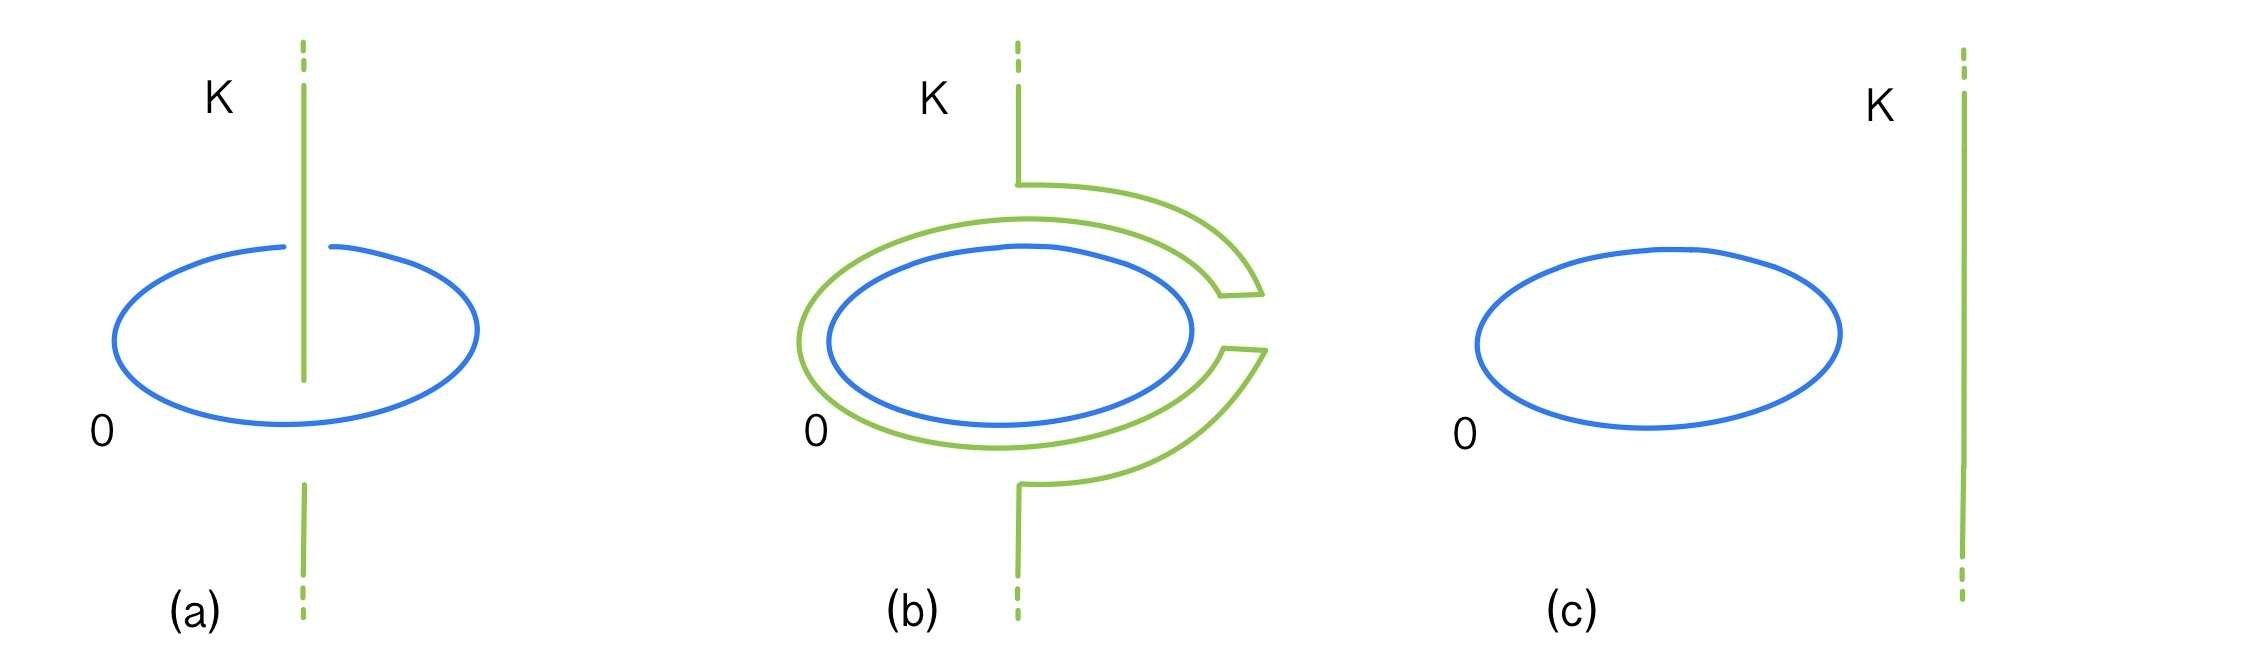
\includegraphics[scale=0.2]{figures/squish.jpeg}
    \caption{Unlinking $K$ from a $0$-framed $2$-handle}
    \label{fig:squish}
\end{figure}
When the $2$-handle is knotted, then the problem could get way harder. However, if $K$ transversely intersects the core of the $2$-handle in one point, then the light bulb trick comes in clutch.
\begin{thm}Let $K \subseteq \s^1 \times \s^2$ be a knot intersecting $\{x\} \times \s^2$ transversely in one point $(x, y)$. Then $K$ is isotopic to $\s^1 \times \{y\}$ via an isotopy fixing $\{x\}\times \s^2$.
\end{thm}
\begin{ex}
The following figure shows how to undo a crossing. The main idea is to slide a piece of knot all the way down to the sphere and then send it back up.
\end{ex}
\begin{figure}[H]
    \centering
    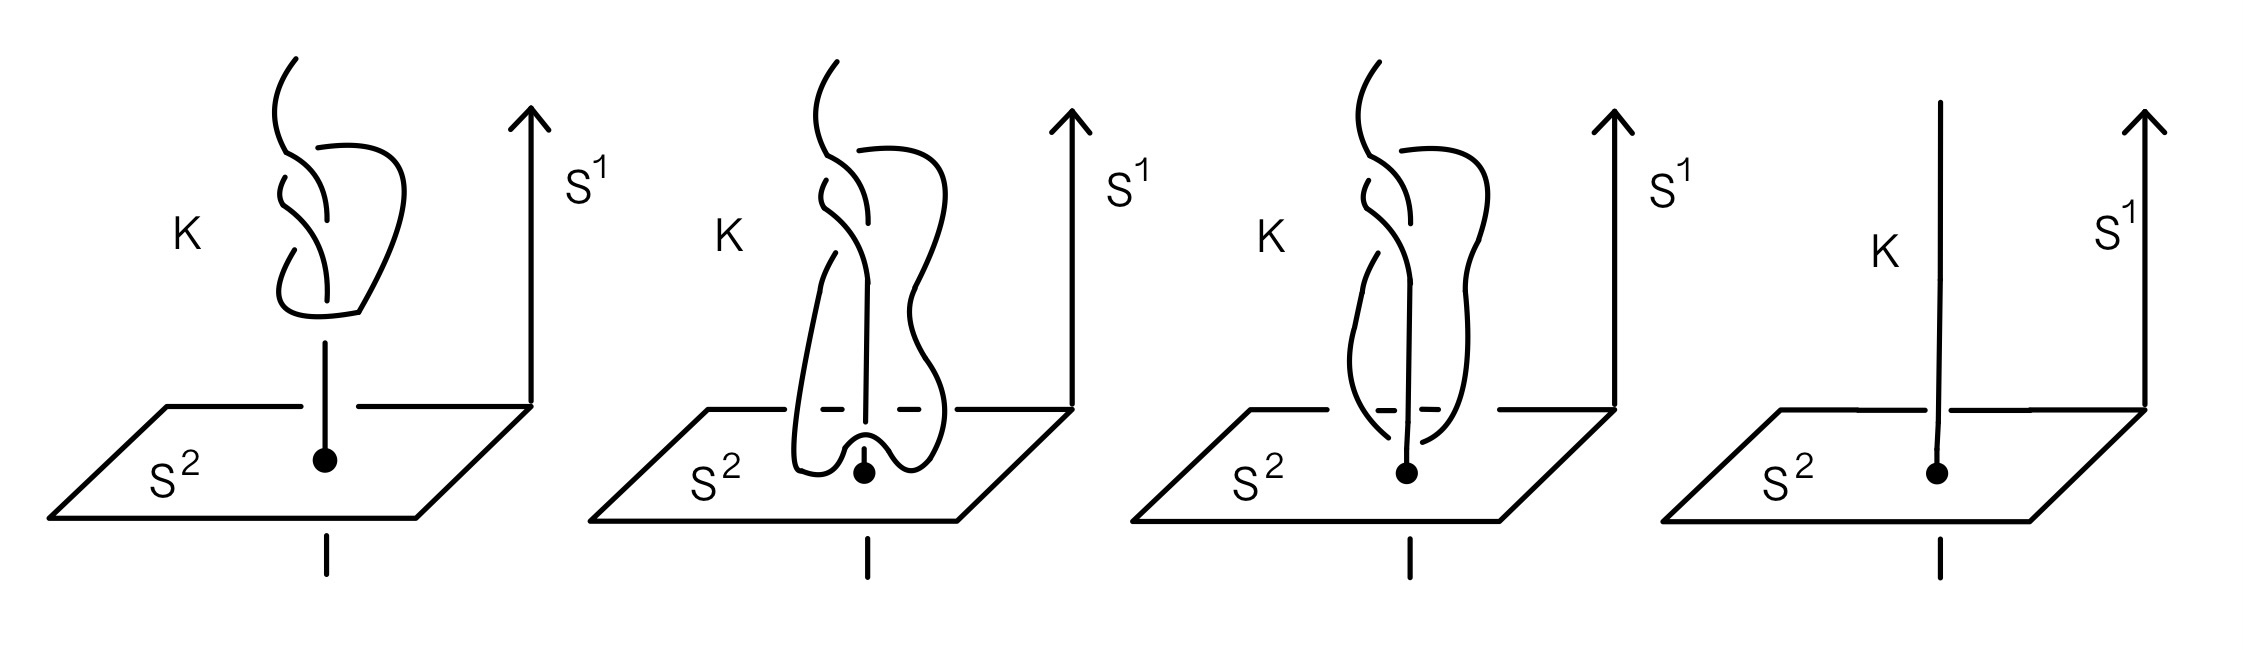
\includegraphics[scale=0.2]{figures/lbt.jpeg}
    \caption{Light bulb trick}
    \label{fig:lbt}
\end{figure}
\section{Ribbon Disks Complement}\label{acqua}
In this section, we outline an algorithm to find the Kirby diagram of a ribbon disk exterior in $\B^4$. We recall the definition for context.
\begin{defn}A disk embedded in $\B^4$ is ribbon if it has no local maxima with respect to the radial height.
\end{defn}
Thus we can visualize a ribbon disk as a finite collection of unknotted disks with some bands attached. \\
Let $K \subseteq \s^3$ be a ribbon knot bounding $D$. 
By performing ribbon moves (band surgeries), we turn $K$ into a collection of disjoint unknotted circles $\{C_i\}_{i=1}^k$ which bound (unknotted) disks $\{D_i\}_{i=1}^k$. For $i = 1 \dots k$, we carve out $D_i$ by placing a dot on $C_i$, as discussed in section \ref{driii}.
\begin{obs}The inverse of the ribbon moves define a cobordism between $\#_1^k(\s^1 \times \s^2)$ and $\s^3 \setminus K$.
\end{obs}
 Each time a circle is merged with another, it creates a $0$-framed $2$-handle in $\B^4 \setminus D$, attached as in Figure \ref{fig:carve}(c) \cite{akbulut2001four}.
\begin{figure}[H]
    \centering
    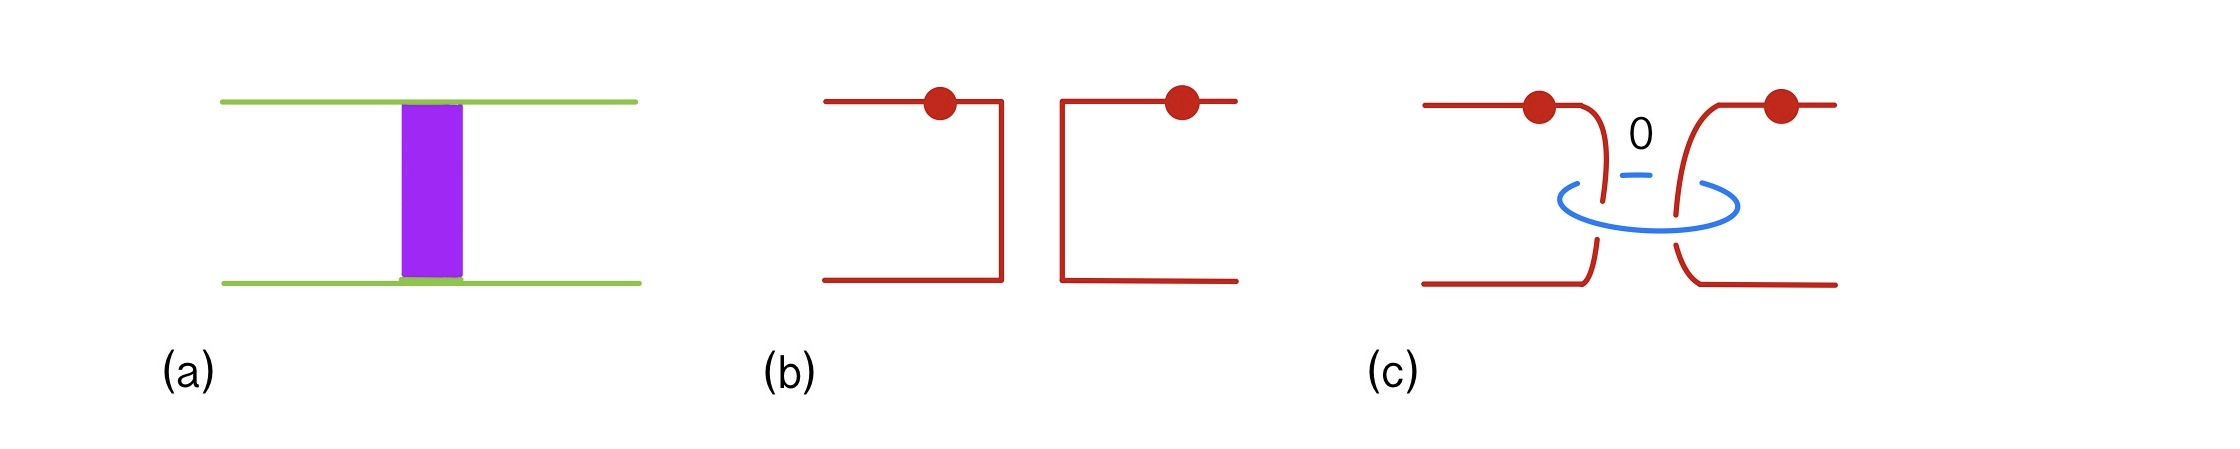
\includegraphics[scale=0.2]{figures/carve.jpeg}
    \caption{Carving a ribbon disk}
    \label{fig:carve}
\end{figure}
\section{A Recipe to Compute the Fundamental Group}\label{rec}
Let $\mathfrak{k}$ be a Kirby diagram of $X$. In this section we describe a procedure to compute the fundamental group of $X$ from $\mathfrak{k}$.
It is well known that a handle decomposition carries a CW complex structure. Collapsing a $k$ handle $\D^k \times \D^{n-k}$ onto the core $\D^k \times 0$, gives rise to a $k$ cell \cite{benedetti2019lectures}. 
\begin{ex}Let $X = \B^4 \cup_1^{n_1}H_1^i$ Then $$
X \sim \vee_1^{n_1} \s^1
$$where each $S^1$ is the core of a $1$-handle. 
\end{ex}
Now we explain how to obtain a presentation of $\pi_1(X)$. For more details, we refer the reader to \cite{saveliev2012}.
\begin{rem}
In general $\pi_1(X)$ is determined by the union of handles of index $\leq 2$.
\end{rem}
\textbf{Procedure}: 
\begin{itemize}
    \item Choose orientations on the attaching spheres,
    \item The generators are the $1$-handles represented as core curves,
    \item The relations are specified by the oriented attaching $\s^1$ of the $2$-handles, written as words of the generators (up to homotopy).
\end{itemize}
\begin{rem}The framing coefficients of the $2$-handles are immaterial.
\end{rem}
We provide two examples, one of which involves the dotted circle notation.
\begin{ex}
\begin{figure}[H]
    \centering
    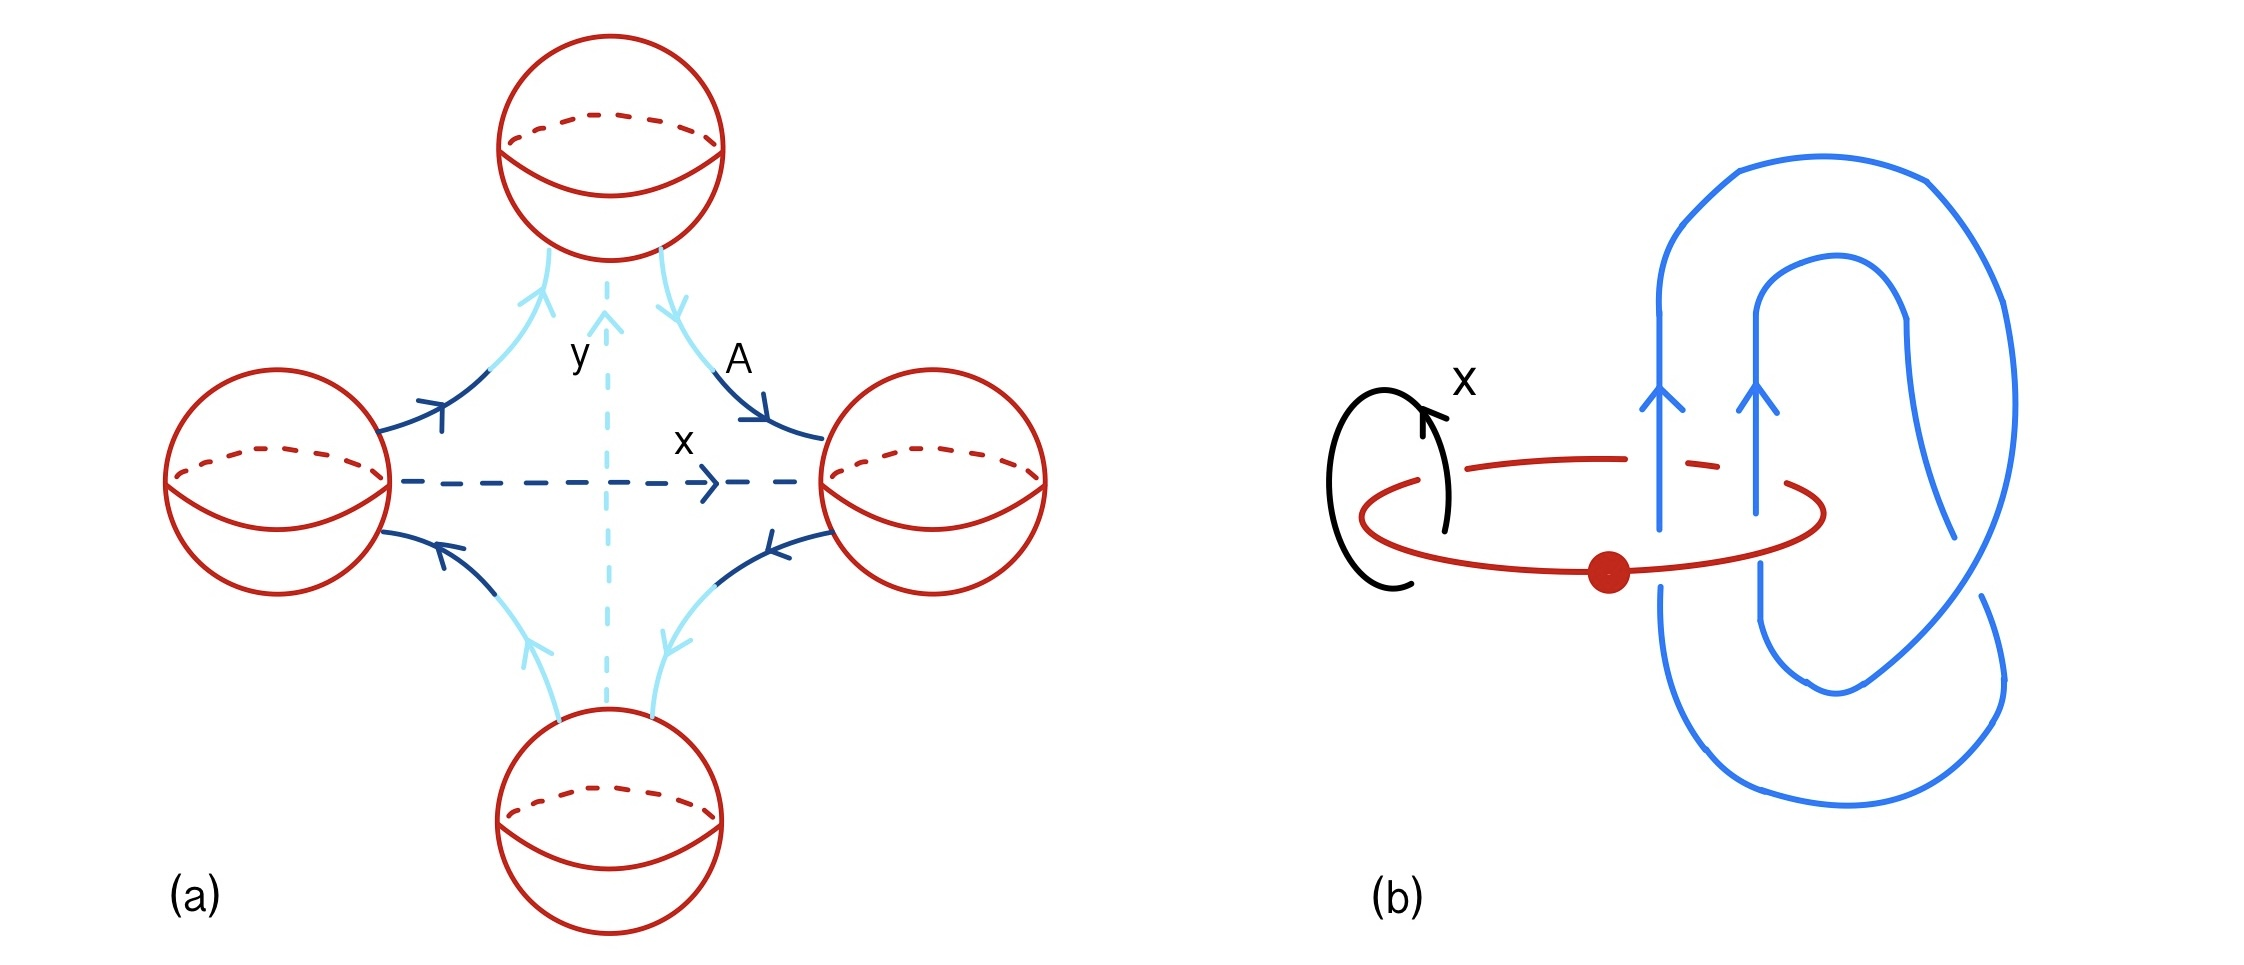
\includegraphics[scale=0.2]{figures/ex_pi1.jpeg}
    \caption{Fundamental group computation}
    \label{fig:funda}
\end{figure}
Consider Figure \ref{fig:funda}(a). Starting from the point A, we obtain the following presentation : $$
\pi_1(X) = \langle x, y \quad | \quad xyx^{-1}y^{-1} \rangle \cong \Z \oplus \Z
$$
Whereas from the diagram \ref{fig:funda}(b), we deduce the following presentation: $$
\pi_1(X) = \langle x \quad | \quad x^2 \rangle = \Z/2\Z
$$
\end{ex}
\section{A Glance at Double Branched Covers}\label{covers}
In this section we prove the existence and uniqueness of the double branched cover of $\B^4$ along an embedded disk $D$, then we sketch an algorithm to draw its Kirby diagram. \\ \\
We recall the general definition for context. Let $M$ be a $4$-manifold.
\begin{defn}
A double branched covering is a proper map $f :N \rightarrow M$ with critical set $B$, called the branch locus, such that:  \\
(i) $f|_{N \setminus f^{-1}(B)} : N \setminus f^{-1}(B) \rightarrow M \setminus B$
is a double covering. \\
(ii) On $f^{-1}(B)$, $f$ is locally defined as $$
\C \times \R_{+}^2 \rightarrow \C \times \R_{+}^2
$$ $$ (z, x) \rightarrow (z^2, x)
$$
\end{defn}
We examine the basic example where $M = \B^4$ and $B$ is an embedded ribbon disk. 
The same techniques apply in similar settings.
\begin{lem} $H_1(\B^4\setminus D) \cong \Z$
\end{lem}
\proof
Consider a open tubular neighbourhood $\nu(D) \cong D \times \B^2$. By Mayer Vietoris' exact sequence, we have: $$
\begin{tikzcd}
0 \arrow[r] & H_1(\nu(D) \setminus D) \arrow[r] & H_1(\B^4 \setminus D)\oplus H_1(\nu(D)) \arrow[r] & 0
\end{tikzcd}
$$
Therefore $H_1(\B^4 \setminus D)\cong \Z$, as desired.
\endproof
By Hurewicz theorem, there exists a surjective homomorphism $\pi_1(\B^4\setminus D) \rightarrow H_1(B^4\setminus D) \cong \Z$. Thus, there exists a unique index $2$ subgroup of $\pi_1(\B^4 \setminus D)$.
This proves the existence and uniqueness of the double covering of $\B^4 \setminus D$. 
Then we locally extend such double covering near the branch locus, in a way that satisfies the local property. The uniqueness of the latter extension follows from the topological fact that a $\s^1$ bundle can be uniquely filled by a $\D^2$ bundle. \\ We denote the double branched covering of $\B^4$ along $D$ as $\Sigma(\B^4, D)$.
\\ 
In section \ref{buffet}, we outline a strategy to draw a Kirby diagram for $\Sigma(\B^4, D)$, providing a concrete example.